\documentclass{beamer}

\usepackage[utf8]{inputenc}
\usepackage{amsmath}
\usepackage{amsfonts}
\usepackage{amssymb}
\usepackage{graphicx}
\usepackage{tikz}
\usepackage{hyperref}

\graphicspath{{../}{./}{../images/}{./images/}}

% ===== KCPC clean theme =====
\usetheme{default}
\useinnertheme{rectangles}
\useoutertheme{default}

\setbeamertemplate{navigation symbols}{}

% --- Colours ---
\definecolor{kcpc-bg}{RGB}{250,250,250}
\definecolor{kcpc-text}{RGB}{20,20,20}
\definecolor{kcpc-muted}{RGB}{90,90,90}
\definecolor{kcpc-red}{RGB}{176,0,0}

\setbeamercolor{background canvas}{bg=kcpc-bg}
\setbeamercolor{normal text}{fg=kcpc-text}
\setbeamercolor{frametitle}{fg=kcpc-text,bg=kcpc-bg}
\setbeamercolor{title}{fg=kcpc-text}
\setbeamercolor{subtitle}{fg=kcpc-muted}
\setbeamercolor{structure}{fg=kcpc-red}

\setbeamerfont{title}{series=\bfseries,size=\Large}
\setbeamerfont{frametitle}{series=\bfseries,size=\large}

\setlength{\parskip}{0.4em}

\setbeamertemplate{itemize item}{$\rightarrow$}
\setbeamertemplate{itemize subitem}{$\rightarrow$}

\setbeamertemplate{headline}{
    \vspace{0.2cm}
    \hspace{0.2cm}
    \textcolor{kcpc-muted}{\small\insertsection}
    \hfill
}

\setbeamertemplate{footline}{
    \hspace{0.2cm}
    \textcolor{kcpc-muted}{\small KCPC}
    \hfill
    \vspace{0.3cm}
}

\setbeamertemplate{background}{
    \begin{tikzpicture}[remember picture,overlay]
        \node[
            opacity=0.035,
            at=(current page.center)
        ] {
            
\includegraphics[width=0.55\paperwidth]{kcpc-logo.png}
        };
    \end{tikzpicture}
}

\AtBeginSection[]{
    \begin{frame}[plain]
        \vfill
        \centering
        {\Large\bfseries \insertsection}
        \vfill
    \end{frame}
}

\hypersetup{colorlinks=true,linkcolor=kcpc-red,urlcolor=kcpc-red}

\title{Introduction to Competitive Programming}
\subtitle{So I hear you’d like to do some ranked coding\dots}
\author{King's Competitive Programming Club}
\date{Workshop 1}

\begin{document}

% Slide 1
\begin{frame}[plain]
    \titlepage
\end{frame}

% Slide 2
\begin{frame}{Workshop Agenda}
    \begin{itemize}
        \item What does KCPC do?
        \item Who is KCPC?
        \item What is Competitive Programming?
        \item Why start KCPC?
        \item Why do Competitive Programming?
        \item Some nice problems
        \item Final messages
    \end{itemize}
\end{frame}

% Section 1
\section{Who is KCPC}

\begin{frame}{Who is KCPC}
    King’s Competitive Programming Club:
    \vspace{0.5em}
    \begin{itemize}
        \item President: Matthew
        \pause
        \item Vice President: Kutay
        \pause
        \item General Secretary and Treasurer: Annoor (Beed)
        \pause
        \item Competitive Programmes: Marcell
        \pause
        \item In collaboration with KCL Tech!
        \pause
        \item Partnered with Orthant Research Group under the Orthant Research Europe division
    \end{itemize}
\end{frame}

% Section 2
\section{Why start KCPC?}

\begin{frame}{Why start King’s Competitive Programming Club?}
    \begin{itemize}
        \item Create a central hub for algorithmic training in London
        \pause
        \item Provide structured, high-quality training
        \pause
        \item Replace isolated practise with community learning
        \pause
        \item Develop elite algorithmic thinkers
        \pause
        \item Connect students to top-tier opportunities
        \pause
        \item Treat competitive programming as a serious discipline
        \pause
        \item Build a cross-University collaborative network
    \end{itemize}
\end{frame}

% Section 3
\section{What does KCPC do?}

\begin{frame}{What does KCPC do?}
    \begin{itemize}
        \item Run weekly training sessions
        \pause
        \item Teach algorithm and data structures
        \pause
        \item Host competitive programming contests
        \pause
        \item Train competition teams
        \pause
        \item Provide mentoring and coaching
        \pause
        \item Support all skill levels
        \pause
        \item Maintain an active collaborative community
    \end{itemize}
\end{frame}

% Section 4
\section{What is Competitive Programming?}

\begin{frame}{What is Competitive Programming?}
    \begin{itemize}
        \item A \textbf{sport} focused on solving challenging problems
        \pause
        \item Problems are solved via correct and efficient \textbf{algorithms}
        \pause
        \item Must adhere to \textbf{constraints} to score points
        \pause
        \item Requires both \textbf{designing} and \textbf{implementing} algorithms
        \pause
        \item Timed competitions are held \textbf{online} or at \textbf{LAN} events
        \pause
        \item Solutions are judged automatically on submission
        \pause
        \item Competitions are timed
    \end{itemize}
\end{frame}

% Section 5
\section{What is a correct and efficient algorithm?}

\begin{frame}{What is a correct and efficient algorithm?}
    \begin{itemize}
        \item Sound: For all solutions given by an algorithm is indeed correct
        \pause
        \item Complete: An algorithm finds a solution when one exist
        \pause
        \item Fast: An algorithm terminates within the allotted time
        \pause
        \item Small: An algorithm only uses the memory allowed
        \pause
        \item Making algorithms sound and complete are relatively easy once you understand the problem
        \pause
        \item But creating them to be fast and small is where most of the challenges lie.
    \end{itemize}
\end{frame}

% Section 6
\section{Requirements for designing algorithms}

\begin{frame}{Requirements for designing algorithms}
    \begin{itemize}
        \item Strong foundations in \textbf{mathematics}
        \pause
        \item Algorithmic \textbf{analysis}
        \pause
        \item Knowledge of \textbf{algorithm theory}
        \pause
        \item Ability to use \textbf{well-known techniques}
        \pause
        \item \textbf{Creativity} to develop new insights and ideas
        \pause
        \item Awareness of how algorithms related to \textbf{scientific research}
        \pause
        \item Don’t worry if this seems too much, you only need GCSE level mathematics to get started!
    \end{itemize}
\end{frame}

% Section 7
\section{Requirements for implementing algorithms}

\begin{frame}{Requirements for implementing algorithms}
    \begin{itemize}
        \item Good algorithm design
        \pause
        \item Strong programming skills: C++, Python, Java
        \pause
        \item Ability to translate ideas into correct code
        \pause
        \item Attention to detail in handling test cases
        \pause
        \item You won’t need to make the code maintainable like in software engineering.
        \pause
        \item But most solutions are at most a few hundred lines of codes anywhere so making your solution concise and straightforward.
    \end{itemize}
\end{frame}

% Section 8
\section{Example of a Competitive Programming problem}

\begin{frame}{Ex: Problem description}
    \centering
    \url{https://codeforces.com/problemset/problem/231/A}
    \par\vspace{0.3em}
    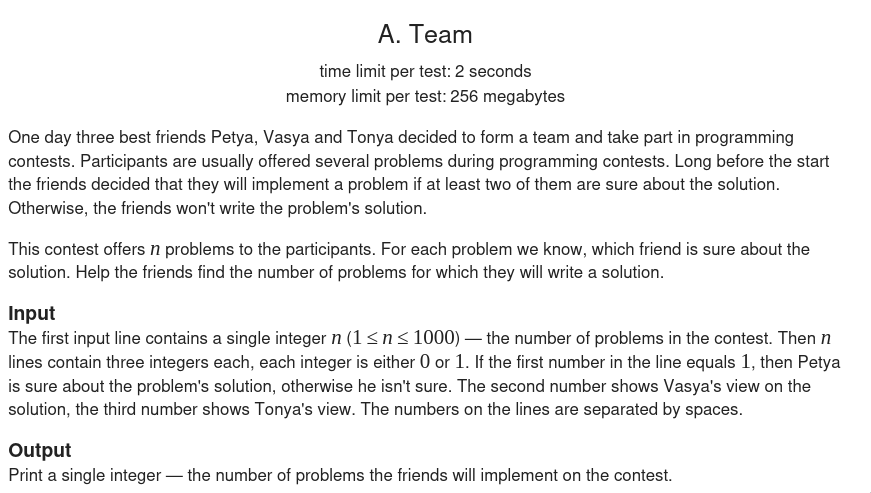
\includegraphics[width=0.88\textwidth,height=0.62\textheight,keepaspectratio]{cf_231a_desc.png}
\end{frame}

\begin{frame}{Ex: Input and Output}
    \centering
    \url{https://codeforces.com/problemset/problem/231/A}
    \par\vspace{0.3em}
    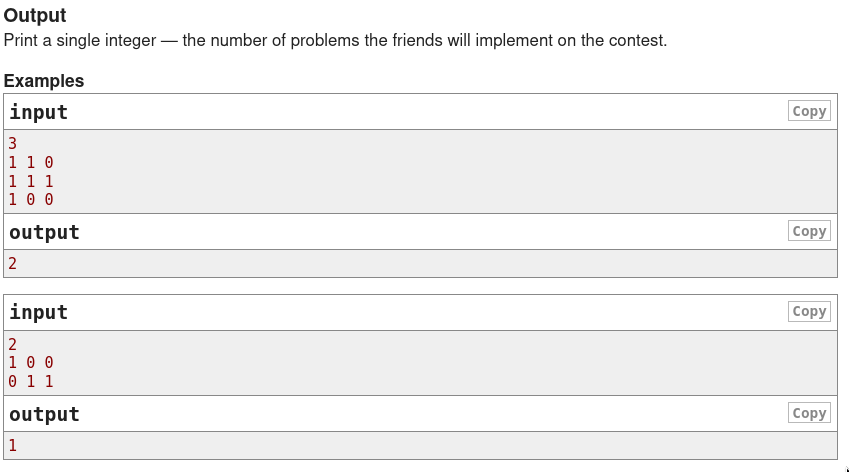
\includegraphics[width=0.88\textwidth,height=0.62\textheight,keepaspectratio]{cf_231a_io.png}
\end{frame}

\begin{frame}{Ex: Problem notes}
    \centering
    \url{https://codeforces.com/problemset/problem/231/A}
    \par\vspace{0.5em}
    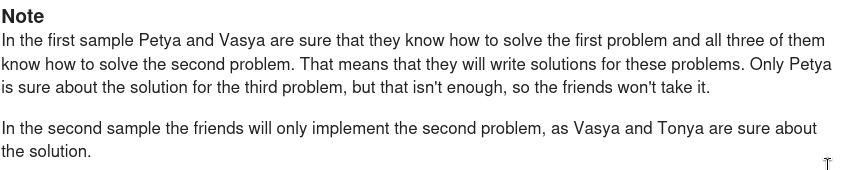
\includegraphics[width=0.88\textwidth,height=0.55\textheight,keepaspectratio]{cf_231a_note.png}
\end{frame}

% Section 9
\section{Why do Competitive Programming?}

\begin{frame}{Why do Competitive Programming?}
    \begin{itemize}
        \item Sharpens your problem-solving skills
        \pause
        \item Improves coding accuracy and speed
        \pause
        \item Many companies value competitive programming experience
        \pause
        \item Deepens understanding of algorithms and data structures
        \pause
        \item It’s fun
    \end{itemize}
\end{frame}

% Section 10: Some nice problems
\section{Some nice problems}

\begin{frame}{Some nice problems}
    \begin{columns}[c]
        \begin{column}{0.55\textwidth}
            Problems and materials on GitHub:
            \par\vspace{0.8em}
            {\scriptsize\url{https://github.com/orthant-kcpc/kcpc-workshops/tree/main/KCPC\%20Year\%201\%20Workshops/2nd\%20Semester/Week\%201}}
        \end{column}
        \begin{column}{0.4\textwidth}
            \centering
            
\includegraphics[width=\linewidth,keepaspectratio]{github_qr.png}
        \end{column}
    \end{columns}
\end{frame}

% Section 11: Final messages
\section{Final messages}

\begin{frame}{Final messages}
    \begin{itemize}
        \item \textbf{Too easy today?} Harder challenges are coming
        \pause
        \item \textbf{Too hard today?} That means you’re learning and that's great!
        \pause
        \item Either way, \textbf{you belong here}: Our goal is simple: \textbf{be better than yesterday}
        \pause
        \item See you \textbf{next week} at the \textbf{same time!}
    \end{itemize}
\end{frame}

\end{document}
